\section{Introduction}
\subsection{Background}
\begin{frame}{Introduction}{Background}
\small
\begin{figure}[tb]
  \centering
  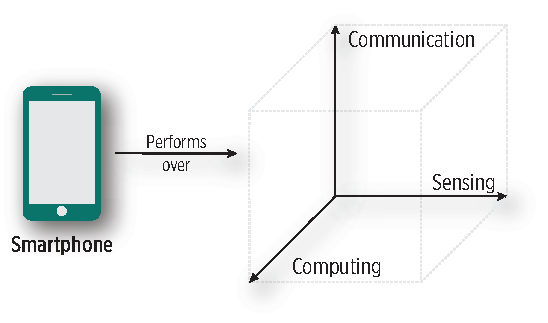
\includegraphics[width=0.4\textwidth]{vectors/smartphone-dimensions-v2}
  \caption{The advances in the communication, computing and sensing dimensions of mobile devices contribute to their acceptance by society.}  
\end{figure}

\begin{block}{\small \textbf{Background}}
\begin{itemize}
	\item Smart devices, such as the smartphone, become popular after the advances on many of its components.
	\item The sensing dimension enables \emph{context-awareness} in mobile device, for new interaction ways with users and enhanced operation.
	\item Battery advances are slower than those of other smartphone components~\cite{Kjaergaard2012}, growing 5-10\% yearly~\cite{Ma2012,Evarts2015}.
	\item The energy constraint is critical when continuous access to sensors is needed, as in \textbf{mobile sensing applications}.
\end{itemize}
\end{block}
\end{frame}

\begin{frame}{Introduction}{Motivation}
\small
\begin{block}{\small \textbf{Motivation}}
\begin{itemize}
	\item For the sensing dimension, scientific efforts have been done for achieving the energy efficiency of the GPS location provider.
	\item The understanding of mobility could augment the location-awareness of the smartphone for many purposes, such as energy savings and the development of Mobility Based Services (MBS).
	\item As a high level of abstraction, mobility can be characterized as a sequence of frequently visited places (stay points).
\end{itemize}
\end{block}
\end{frame}